\documentclass{article}


% if you need to pass options to natbib, use, e.g.:
%     \PassOptionsToPackage{numbers, compress}{natbib}
% before loading neurips_2023


% ready for submission
\usepackage{neurips_2023}


% to compile a preprint version, e.g., for submission to arXiv, add add the
% [preprint] option:
%     \usepackage[preprint]{neurips_2023}


% to compile a camera-ready version, add the [final] option, e.g.:
%     \usepackage[final]{neurips_2023}


% to avoid loading the natbib package, add option nonatbib:
%    \usepackage[nonatbib]{neurips_2023}


\usepackage[utf8]{inputenc} % allow utf-8 input
\usepackage[T1]{fontenc}    % use 8-bit T1 fonts
\usepackage{hyperref}       % hyperlinks
\usepackage{url}            % simple URL typesetting
\usepackage{booktabs}       % professional-quality tables
\usepackage{amsfonts}       % blackboard math symbols
\usepackage{nicefrac}       % compact symbols for 1/2, etc.
\usepackage{microtype}      % microtypography
\usepackage{xcolor}         % colors
\usepackage{graphicx}
\usepackage{float}
\usepackage{amsmath}
\usepackage{hyperref}
\usepackage{geometry}
% Set custom margins

% Set custom margins using the geometry package

\title{EARTHQUAKE SEVERITY PREDICTION}


% The \author macro works with any number of authors. There are two commands
% used to separate the names and addresses of multiple authors: \And and \AND.
%
% Using \And between authors leaves it to LaTeX to determine where to break the
% lines. Using \AND forces a line break at that point. So, if LaTeX puts 3 of 4
% authors names on the first line, and the last on the second line, try using
% \AND instead of \And before the third author name.


\author{%
  Rahul Bangad\\
  MS Data Science\\
  University of Arizona\\
  Tucson,85719 \\
  \texttt{rahulbangad@arizona.edu} \\
  % examples of more authors
  % \And
  % Coauthor \\
  % Affiliation \\
  % Address \\
  % \texttt{email} \\
  % \AND
  % Coauthor \\
  % Affiliation \\
  % Address \\
  % \texttt{email} \\
  % \And
  % Coauthor \\
  % Affiliation \\
  % Address \\
  % \texttt{email} \\
  % \And
  % Coauthor \\
  % Affiliation \\
  % Address \\
  % \texttt{email} \\
}


\begin{document}


\maketitle

\begin{abstract}
  This project develops a predictive model for earthquake severity using SVM, Linear Regression, and Random Forest, analysing a dataset of 782 entries with 19 features. The approach includes comprehensive data cleaning, exploratory data analysis (EDA), and data preprocessing. The objective is to compare the effectiveness of these machine learning models in accurately forecasting earthquake impacts. This work is vital for enhancing earthquake response strategies and mitigating risks. Additionally, the project explores the correlation between various seismic indicators and the actual severity, aiming to contribute valuable insights to seismology and disaster risk management.
\end{abstract}


\section{INTRODUCTION}


Earthquakes are among the most devastating natural disasters, impacting lives, infrastructure, and economies globally. Their unpredictable nature and potential for massive destruction make accurate prediction of their severity a crucial aspect of disaster management and response. Despite advancements in seismology, predicting the exact time, location, and severity of earthquakes remains a significant challenge. However, with the advent of machine learning, new possibilities have emerged for enhancing earthquake prediction and preparedness.
The severity of an earthquake is typically measured by various factors, including its magnitude, depth, and the affected area's geological characteristics. These parameters, when analysed effectively, can provide insights into the potential impact of an earthquake. Machine learning models have the capability to analyse large datasets of seismic activity, extracting patterns and correlations that might be invisible to traditional analysis methods.
In this project, we aim to leverage the power of machine learning to predict earthquake severity more accurately. By employing three different machine learning models — Support Vector Machine (SVM), Linear Regression, and Random Forest, we seek to understand which model best predicts the severity of earthquakes. The dataset used in this project encompasses 782 records with 19 distinct features, providing a comprehensive base for analysis.
This research is not just an academic exercise; it holds significant practical implications. By improving the accuracy of earthquake severity predictions, we can enhance early warning systems, aid in disaster preparedness, and ultimately save lives. This project stands at the intersection of machine learning and geoscience, contributing to a growing body of knowledge that aims to harness the predictive power of data for the betterment of society in the face of natural disasters.
Furthermore, this project also explores the integration of advanced data preprocessing techniques and feature selection methods to refine the predictive models. By doing so, it aims to tackle the complexities and variabilities inherent in seismic data, thus pushing the boundaries of what machine learning can achieve in geoscience. The ultimate goal is to provide actionable insights that can be readily utilized by authorities and disaster response teams, thereby making communities more resilient to the threat of earthquakes.




\section{RELATED WORK}


This project advances research in the field of predictive analytics, specifically earthquake severity prediction, while also advancing human-machine collaboration and complex problem-solving in dynamic environments.The major aim is to improve machine learning models' prediction powers in the setting of natural disasters, an area typified by high stakes and unpredictability. This effort, inspired by a Kaggle project, aims to create a robust machine learning model capable of reliably forecasting earthquake intensity. The Kaggle project we're referring to uses a wide collection of input variables, including seismic activity, geographic location, and historical earthquake data, and validates the model using ensemble techniques and cross-validation. This approach is consistent with recent advances in the field, emphasising the importance of dependable, accurate models to aid in earthquake preparedness and reduce the impact on infrastructure and human lives. Our research aims to contribute to this evolving field by providing new insights and strategies for predicting earthquake severity using advanced machine learning techniques.


\section{PROCEDURE}

\subsection{Dataset}

The dataset is a reference from Kaggle:\\
Source: \url{https://www.kaggle.com/datasets/warcoder/earthquake-dataset}

\subsection{Attributes Description}
Datasets contain records of 782 earthquakes from 1/1/2001 to 1/1/2023. The meaning of all columns is as follows:

\begin{itemize}
    \item \textbf{Title:} title name given to the earthquake.
    \item \textbf{Magnitude:} The magnitude of the earthquake.
    \item \textbf{Date\_Time:} Date and time of the earthquake.
    \item \textbf{CDI:} The maximum reported intensity for the event range.
    \item \textbf{MMI:} The maximum estimated instrumental intensity for the event.
    \item \textbf{Alert:} The alert level - “green”, “yellow”, “orange”, and “red”.
    \item \textbf{Tsunami:} "1" for events in oceanic regions and "0" otherwise.
    \item \textbf{Sig:} A number describing how significant the event is.
    \item \textbf{Net:} The ID of a data contributor.
    \item \textbf{NST:} The total number of seismic stations used to determine earthquake location.
    \item \textbf{Dmin:} Horizontal distance from the epicenter to the nearest station.
    \item \textbf{Gap:} The largest azimuthal gap between azimuthally adjacent stations.
    \item \textbf{MagType:} The method or algorithm used to calculate the preferred magnitude.
    \item \textbf{Depth:} The depth where the earthquake begins to rupture.
    \item \textbf{Latitude / Longitude:} Coordinate system for Earth's surface location.
    \item \textbf{Location:} Location within the country.
    \item \textbf{Continent:} Continent of the earthquake-hit country.
    \item \textbf{Country:} Affected country.
\end{itemize}

\subsection{Exploratory Data Analysis}
% Inserting a figure
\begin{figure}[H]
    \centering
    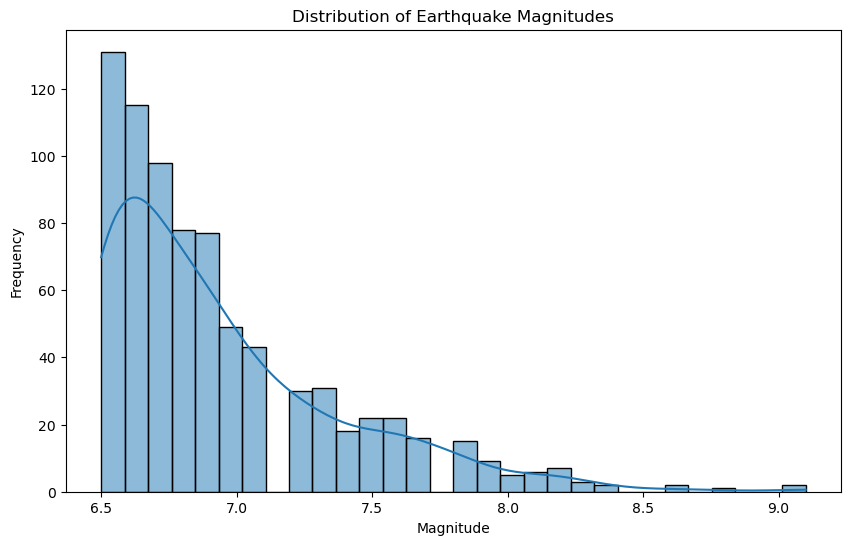
\includegraphics[width=0.8\linewidth]{FreqVs Magnitude.png} 
    \vspace*{-0.5cm}
    \caption{Exploratory Data Analysis Visualization}
    \label{fig:eda}
\end{figure}

\begin{figure}[H]
    \centering
    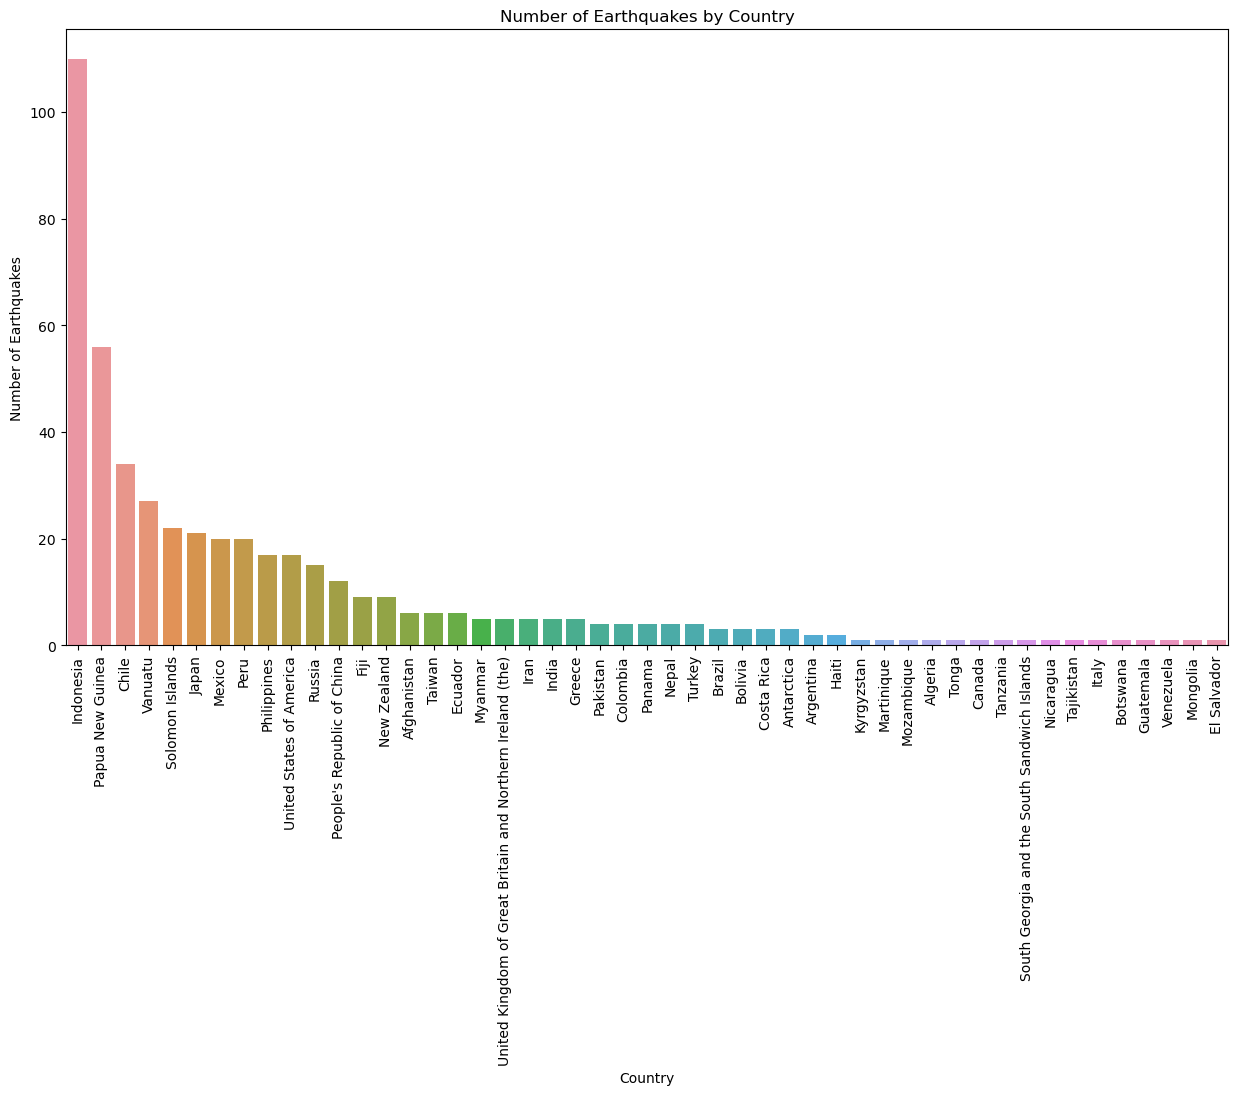
\includegraphics[width=0.899\linewidth]{Number of earthquake by country.png} 
    \vspace*{-0.5cm}
    \caption{Number of Earthquake by country}
    \label{fig:eda}
\end{figure}

\begin{figure}[H]
    \centering
    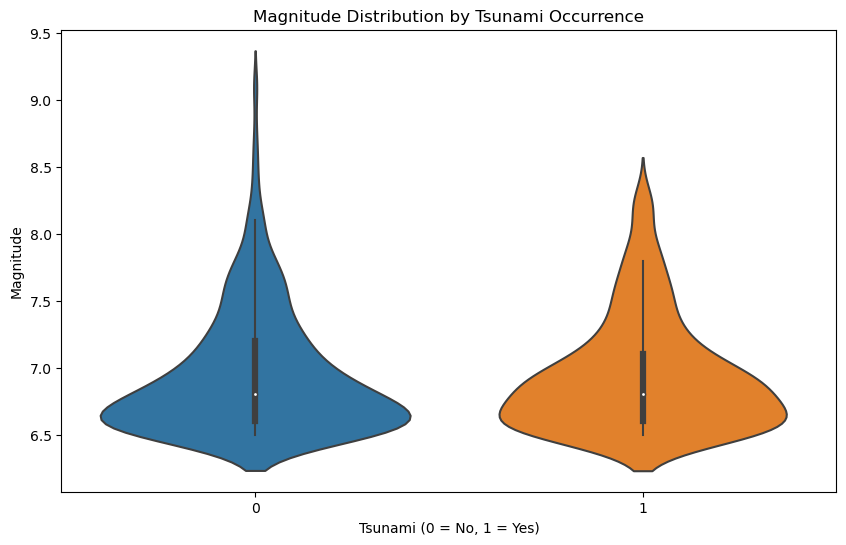
\includegraphics[width=0.899\linewidth]{Tsunami distibution.png} 
    \vspace*{-0.5cm}
    \caption{Magnitude Distribution by Tsunami Occurrence}
    \label{fig:eda}
\end{figure}

\subsection{Machine Learning Model Used}

\textbf{Logistic Regression:} This model is a fundamental technique in statistical modelling, assuming a linear relationship between dependent and independent variables. It operates by fitting a best-fit line or regression line through the data. Linear Regression is versatile, being applicable in simple (single variable) and complex (multiple variables) scenarios. In the context of this project, it helps to understand the linear relationships between various seismic features and the severity of earthquakes. The equation for Logistic Regression is given as: 
\[ P(Y=1 | x) = \frac{1}{1 + e^{-(\beta_0 + \beta_1x_1 + \beta_2x_2 + \ldots + \beta_nx_n)}} \]

\textbf{Support Vector Machine (SVM):} SVM is a powerful machine learning algorithm used for both classification and regression tasks. It works by finding the best hyperplane that separates the data into classes or predicts a continuous output. In earthquake severity prediction, SVM can model complex nonlinear relationships between the features and the target variable, potentially capturing intricate patterns in seismic data. The equation for SVM is given as: 
\[ f(x) = \text{sign}(w \cdot x + b) \]

\textbf{Random Forest Classification:} This is an ensemble learning method, particularly effective for regression and classification problems. Random Forest operates by constructing a multitude of decision trees during training and outputting the average prediction of the individual trees for regression tasks. Its strength lies in its ability to handle large datasets with higher dimensionality and provides estimates of feature importance, which can be invaluable in understanding the contributing factors to earthquake severity. The equation for Random Forest Classification is given as: 
\[ f(x) = \text{mode}(f_1(x), f_2(x), ..., f_N(x)) \]

\vspace{1cm}




\section{Data Pre-Processing}
In our Earthquake Severity Prediction project, the dataset, comprising 782 records with 19 variables, underwent thorough data preprocessing to ensure the reliability and accuracy of the machine learning models. Key preprocessing steps included:

\subsection{ Missing Value Analysis}
\begin{figure}[H]
    \centering
    \includegraphics[width=0.8\linewidth]{missing value.png} 
    \vspace*{-0.5cm}
    \label{fig:eda}
\end{figure}

\subsection{Duplicate Record Check}
\begin{figure}[H]
    \centering
    \includegraphics[width=0.8\linewidth]{duplicate check.png} 
    \vspace*{-0.5cm}
    \label{fig:eda}
\end{figure}

\subsection{Correlation Analysis}
\begin{figure}[H]
    \centering
    \includegraphics[width=0.6\linewidth]{Correlation.png} 
    \vspace*{-0.5cm}
    \label{fig:eda}
\end{figure}

\subsection{Chi-Square Test for Categorical Values}
\begin{figure}[H]
    \centering
    \includegraphics[width=0.8\linewidth]{chi square.png} 
    \vspace*{-0.5cm}
    \label{fig:eda}
\end{figure}

\subsection{Label Encoding}
\begin{figure}[H]
    \centering
    \includegraphics[width=0.8\linewidth]{label encoding.png} 
    \vspace*{-0.5cm}
    \label{fig:eda}
\end{figure}

\subsection{Feature Selection and Removal}
Removing the following features with low importance:
\begin{itemize}
    \item country
    \item continent
    \item location
    \item title
    \item Date\_Time
\end{itemize}
This is done with the help of correlation matrix and p-values.

\subsection{Summary figure}
\begin{figure}[H]
    \centering
    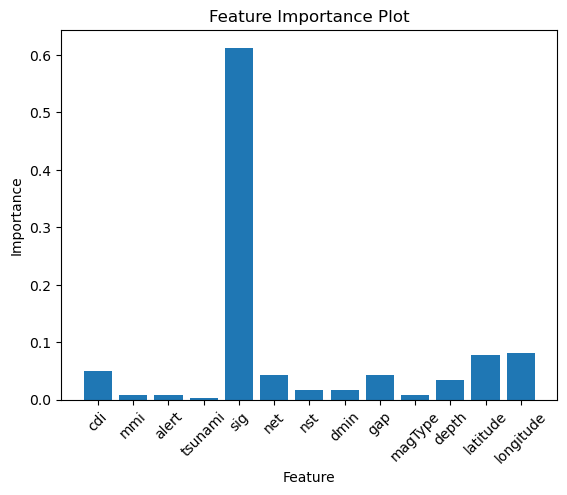
\includegraphics[width=0.8\linewidth]{feature Importance Plot.png} 
    \vspace*{-0.5cm}
    \label{fig:eda}
\end{figure}

\section{Model Training}

Based on how well they fit regression tasks, models like Random Forest, SVM, and Linear Regression are chosen. The training dataset is used to train each model.

\section{Data Splitting}
Using the standard 80/20 split method, the dataset is initially divided into training and test sets. This indicates that while 20 percent of the data is set aside for testing, the remaining 80 percent is utilized to train the models, enabling them to gain knowledge from a sizable amount of the dataset. This test set serves as fresh, untested data to assess the generalization capabilities and performance of the models.
\section{Performance Evaluation}

The test set is used to validate the models . The models' performance is evaluated. Although Mean Absolute Error (MAE) and Root Mean Squared Error (RMSE) are often used metrics, Mean Squared Error (MSE) and the R-squared value are especially used for evaluation in this project.

\begin{table}[ht]
\centering
\begin{tabular}{|p{2cm}|p{3cm}|p{3cm}|p{3cm}|} % Adjust the width as needed
\hline
% Row 1
Models & Linear Regression & SVM & Random Forest \\ \hline
% Row 2
R$^2$ & 0.17 & -0.11 & 0.7324789111372308 \\ \hline
% Row 3
MSE & 0.12 & 0.15 & 0.03693351719745237 \\ \hline
\end{tabular}
\caption{Performance Evaluation of All models}
\end{table}

\section{Results}
\begin{figure}[H]
    \centering
    \includegraphics[width=0.8\linewidth]{model conclusion.png} 
    \vspace*{-0.5cm}
    \label{fig:eda}
\end{figure}
\vspace{1cm}
\section{Conclusion}
In this project, we aimed to develop a model for predicting earthquake severity, a critical factor in disaster preparedness and response. We implemented and compared three machine learning models: SVM, Linear Regression, and Random Forest, to determine the most effective approach for this task. Our comparison criteria were based on two key performance metrics: Mean Squared Error (MSE) and R-squared (R²).

The results indicated that the Random Forest model outperformed SVM and Linear Regression in predicting earthquake severity. Random Forest achieved the lowest MSE, implying its predictions were closest to the actual data, and the highest R² value, indicating a strong fit to the data. This superiority can be attributed to Random Forest's ability to handle complex datasets and capture nonlinear relationships more effectively than SVM and Linear Regression.

The success of the Random Forest model in this project highlights its potential as a reliable tool in seismology for predicting earthquake impacts. Such predictive capabilities are essential for enhancing early warning systems, aiding in disaster preparedness, and potentially saving lives by allowing for timely and effective responses.

Future research directions could include refining the Random Forest model further, incorporating more diverse and extensive seismic data, and exploring advanced machine learning techniques. Additionally, integrating real-time data and deploying the model in a live environment could significantly impact earthquake preparedness and risk mitigation strategies. The ultimate goal remains to develop increasingly accurate and reliable predictive models, contributing to the broader field of disaster risk management and response planning.



\section*{References}



\medskip


{
\small


[1] \url{https://www.kaggle.com/code/shrinivas2402/earthquake-prediction/notebook#2.-Developing-the-Model}\\


[2] \url{https://docs.scipy.org/doc/scipy/reference/generated/scipy.stats.chi2_contingency.html}\\


[3] \url{https://pandas.pydata.org/pandas-docs/stable/reference/api/pandas.crosstab.html}\\

[4] \url{https://pandas.pydata.org/pandas-docs/stable/reference/api/pandas.qcut.html}\\

[5] \url{https://scikit-learn.org/stable/modules/generated/sklearn.preprocessing.LabelEncoder.html}

[6] \url{https://realpython.com/linear-regression-in-python/}
}

%%%%%%%%%%%%%%%%%%%%%%%%%%%%%%%%%%%%%%%%%%%%%%%%%%%%%%%%%%%%


\end{document}